\documentclass{article}
\usepackage{amsmath,amsthm,amssymb,amsfonts}
\usepackage{setspace,enumitem}
\usepackage{natbib}
\usepackage{afterpage}
\usepackage{booktabs}
\usepackage{pdfpages}
\usepackage{geometry}
\usepackage{graphicx}
\geometry{margin = 1in}
\graphicspath{ {./adjustment/figures/} }

\setlength{\parindent}{0cm}

\newcommand{\R}{\mathbb{R}}


\begin{document}

\section*{FIN 971: Problem Set 2\footnote{Instructor: Dean Corbae}}

Alex von Hafften

\today

\bigskip

Problem outlined in Dean's website.  The profit function and the investment adjustment cost functional forms are:

\begin{align*}
\pi(k_t, z_t) &= z_t k_t^{\theta} \\
\psi(k_{t+1} - (1 -\delta)k_t, k_t) &= \frac{\psi_0 (k_{t+1} - k_t)^2}{2k_t}
\end{align*}

Notice that:

\begin{align*}
\psi(k_{t+1} - (1 -\delta)k_t, k_t) &= \frac{\psi_0 (k_{t+1} - (1 -\delta)k_t + (1 -\delta)k_t - k_t)^2}{2k_t} \\
\implies
\psi(I_t, k_t) 
&= \frac{\psi_0 (I_t + (1 -\delta)k_t - k_t)^2}{2k_t} \\
&= \frac{\psi_0 (I_t -\delta k_t)^2}{2k_t} \\
\psi_I(I_t, k_t) &= \frac{\psi_0 (I_t -\delta k_t)}{k_t} \\
\psi_k(I_t, k_t) &= \psi_0\frac{(I_t - \delta k_t)^2(2) - 2k_t * 2(I_t - \delta k_t)}{(2k_t)^2} \\
&= \psi_0 \frac{I_t^2 - \delta^2 k_t^2}{2k_t^2}
\end{align*}

The model is characterized by the following equations:

\begin{align*}
q_t &= 1 + \frac{\psi_0 (I_t -\delta k_t)}{k_t} \\
q_t &= E_t \Bigg[M_{t+1} \Bigg\{ z_{t+1}\theta k_{t+1}^{\theta - 1}- \psi_0 \frac{I_{t+1}^2 - \delta^2 k_{t+1}^2}{2k_{t+1}^2} + q_{t+1} ( 1 -\delta)\Bigg\} \Bigg] \\
I_t &= k_{t+1} - k_t + \delta k_t \\
c_t &= z_t k_t^{\theta} - \frac{\psi_0 (I_t -\delta k_t)^2}{2k_t} - I_t \\
z_t &= (1 - \rho_z) + \rho_z z_{t-1} + \varepsilon_t \\
M_t &= \frac{1}{1 +r} \Bigg(\frac{c_t}{c_{t-1}}\Bigg)^{-\gamma}
\end{align*}

\pagebreak

\subsection*{1. Steady State}

In steady state, $x_t = x_{t+1} = \bar{x}$ $\forall x$.

\begin{align*}
\bar{z} &= 1\\
\bar{I} &= \delta \bar{k} \\
\bar{q} &= 1\\
\bar{M} &= \frac{1}{1 +r}  \\
\bar{c} &= \bar{k}^\theta - \delta \bar{k}\\
\bar{k} &= \Bigg(\frac{\theta}{r+\delta}\Bigg)^{\frac{1}{1 - \theta}}
\end{align*}

because $\psi(\bar{I}, \bar{k}) = \psi_I(\bar{I}, \bar{k}) = \psi_k(\bar{I}, \bar{k}) = 0$. For the parameter values from the problem set, the steady state values are:

\begin{table}[h!]
  \begin{center}
    \label{tab:table1}
    \begin{tabular}{c|c}
      \hline
      $\bar{z}$ & 1.0 \\
      $\bar{q}$ & 1.0 \\
      $\bar{M}$ & 0.9615\\
      $\bar{k}$ & 77.2351\\
      $\bar{I}$ & 11.5853\\
      $\bar{c}$ & 9.3785\\
    \end{tabular}
  \end{center}
\end{table}

\subsection*{2. Impulse Response Functions}

For $\gamma = 2.0$, the impulse response functions of investment and capital to a one standard deviation shock to productivity.

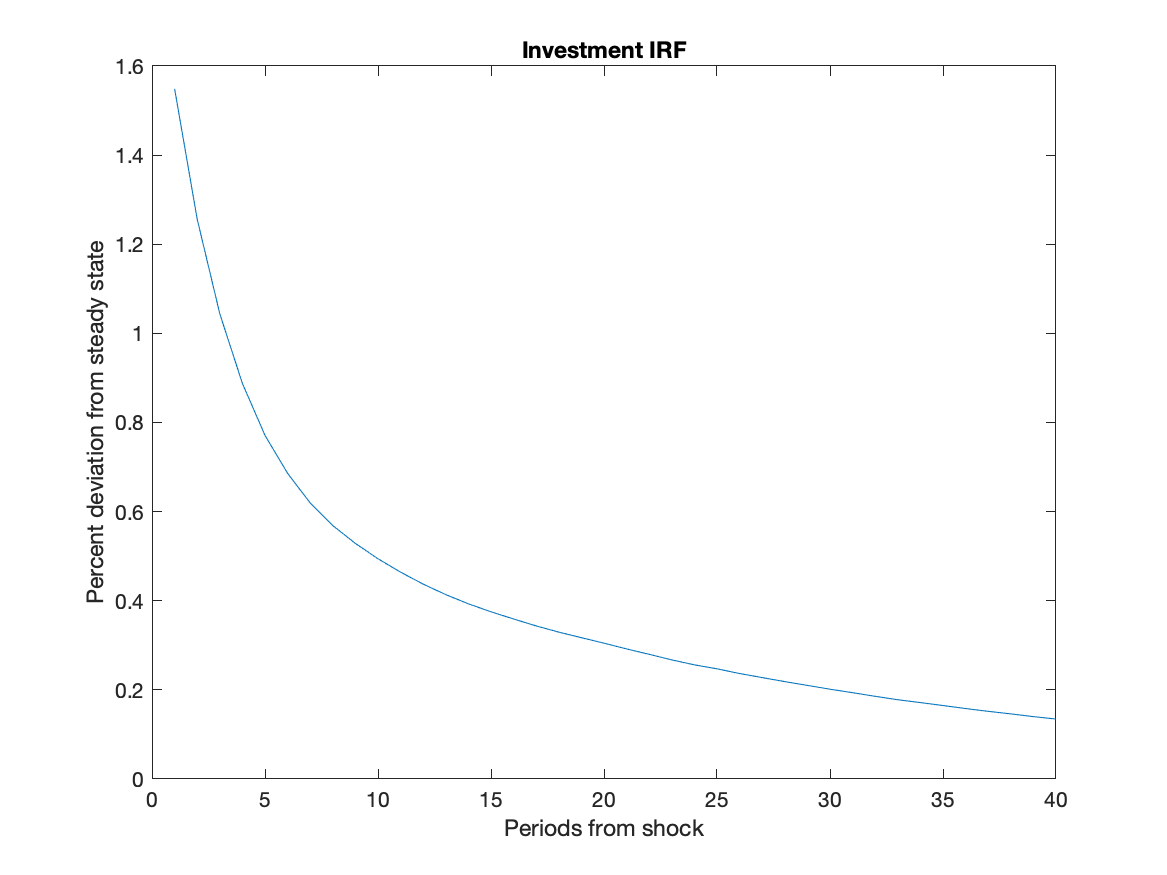
\includegraphics[scale=.6]{p2_i}

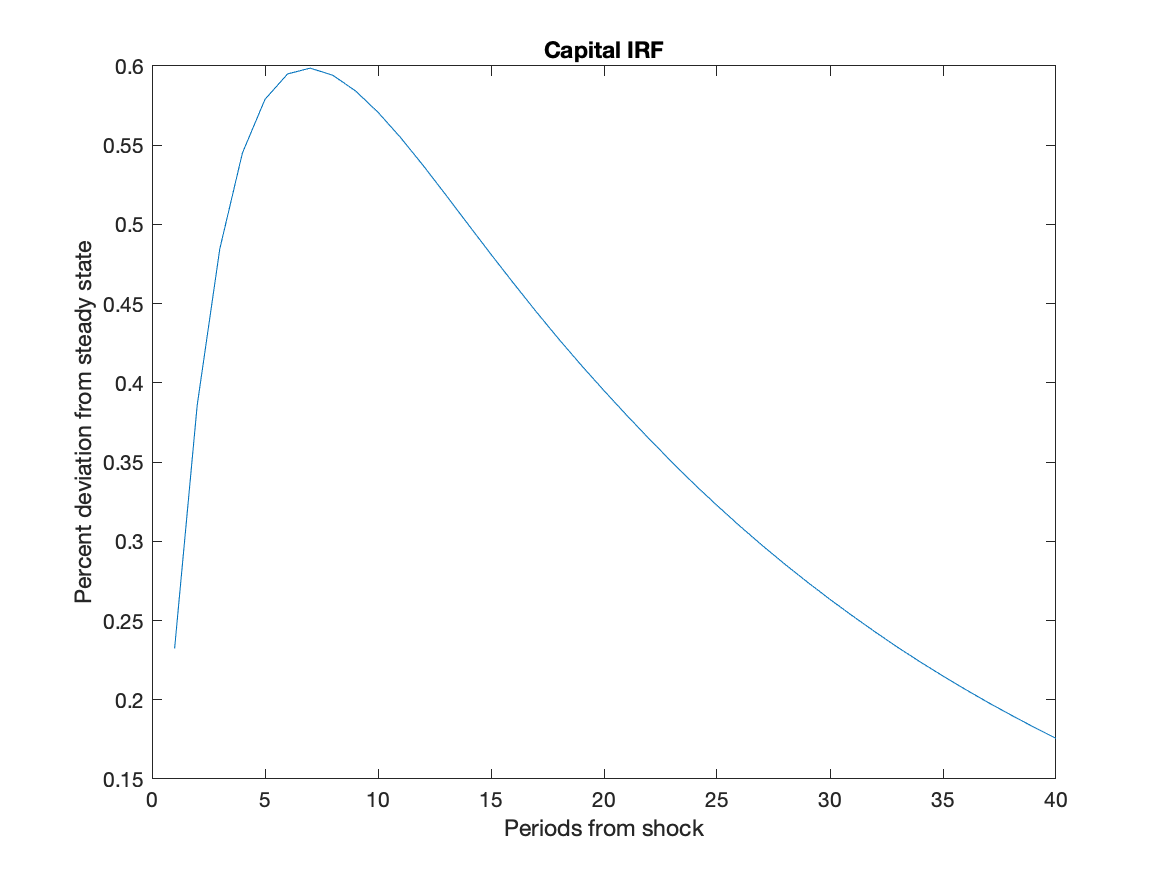
\includegraphics[scale=.6]{p2_k}

For $\gamma = 0.0$, the consumer is risk neutral and with an infinite intertemporal elasticity of substitution.  The consumer does not care about consumption smoothing, so maximizes their total consumption. Thus, they invest everything now that production is more productivity. Thus, capital and investment spike and then return the steady state as productivity returns to the steady state level.

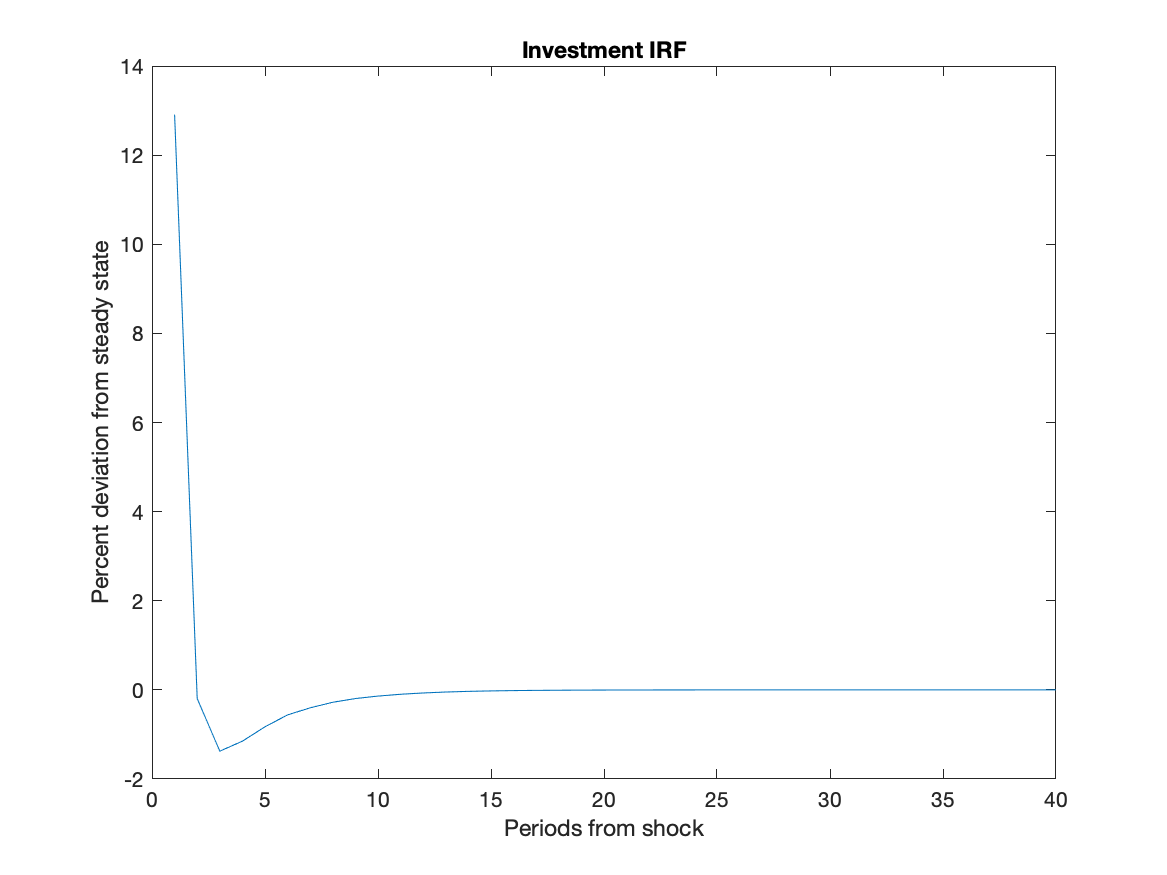
\includegraphics[scale=.6]{p2_i_zero_gamma}

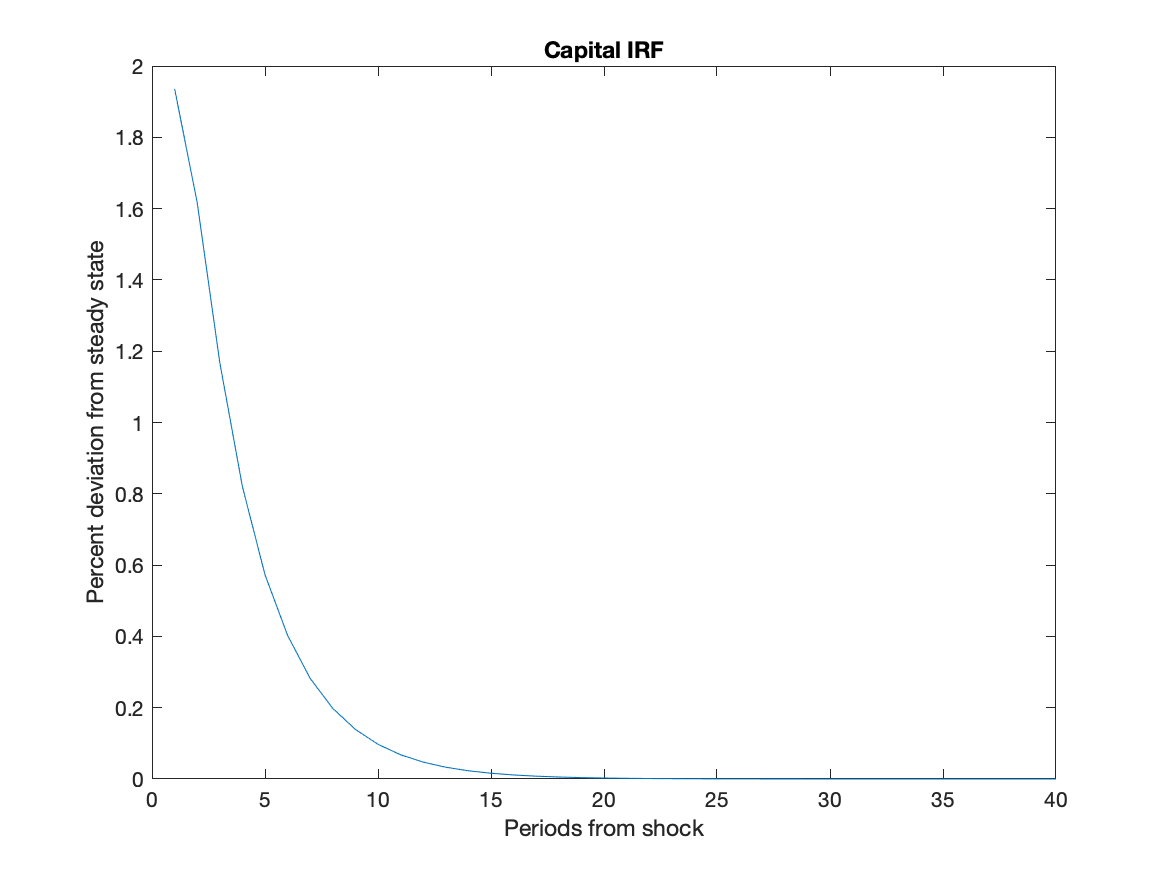
\includegraphics[scale=.6]{p2_k_zero_gamma}

\subsection*{3. Q-Regression}

Running this regression with the simulated data:

$$
\frac{I_t}{k_t} = \alpha + \beta_1 q_{t-1} + \beta_2 \frac{\pi_{t-1}}{k_{t-1}}
$$

I get the following OLS coefficients:

\begin{table}[h!]
  \begin{center}
    \label{tab:table1}
    \begin{tabular}{c|c}
      \hline
      $\alpha$  & -27.9899 \\
      $\beta_1$ & 28.0687 \\
      $\beta_2$ & 0.2624
    \end{tabular}
  \end{center}
\end{table}

Since $q_t$ is always right around 1, I don't think there's much to be gained looking at $\beta_1$.  But $\beta_2$ is positive.  This means that if a firm relatively more profitable, they invest more.

\subsection*{3. Bayesian Estimation with Simulated Data}

I changed ``noadjustment\_est.mod" to include capital adjustment costs.  The following figure shows the priors and posteriors of $\theta, \psi_0, \sigma_\varepsilon, \sigma_q$.  Similar to the no adjustment cost case, the posteriors are very different than the priors, indicating that this model is also well-identified.

\begin{table}[h!]
  \begin{center}
    \label{tab:table1}
    \begin{tabular}{c|ccc}
      Parameter            & Prior Mean & Posterior Mean & 90 \% HPD Interval\\
      \hline
      $\theta$             & 0.5      & 0.7002         & [0.6989, 0.7012]\\
      $\psi_0$             & 0.5      & 0.1848         & [0.0005, 0.3846]\\
      $\sigma_\varepsilon$ & 0.007    & 0.0110         & [0.0100, 0.0120] \\
      $\sigma_q$           & 0.007    & 0.0107         & [0.0099, 0.0116] 
    \end{tabular}
  \end{center}
\end{table}

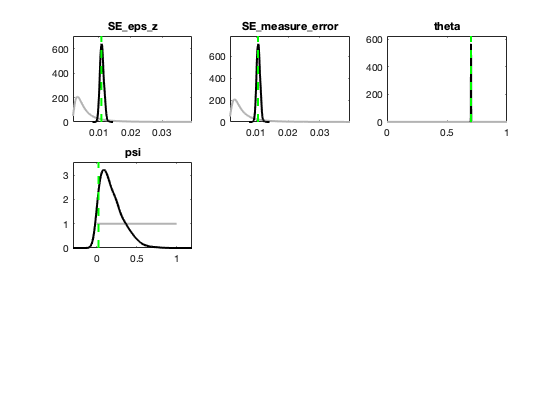
\includegraphics[scale=.8]{p4_priors_posteriors}

\subsection*{4. Bayesian Estimation with Real Data}

I changed ``noadjustment\_est\_D.mod" to include capital adjustment costs.  The following figure shows the priors and posteriors of $\theta, \psi_0, \sigma_\varepsilon, \sigma_q$.

\begin{table}[h!]
  \begin{center}
    \label{tab:table1}
    \begin{tabular}{c|ccc}
      Parameter            & Prior Mean & Posterior Mean & 90 \% HPD Interval\\
      \hline
      $\theta$             & 0.5      & 0.1833         & [0.0335, 0.4150]\\
      $\psi_0$             & 0.5      & 0.0004         & [0.0000, 0.0010]\\
      $\sigma_\varepsilon$ & 78.133   & 114.3764       & [41.4847, 185.1721] \\
      $\sigma_q$           & 0.162    & 0.2595         & [0.2202, 0.2943] 
    \end{tabular}
  \end{center}
\end{table}

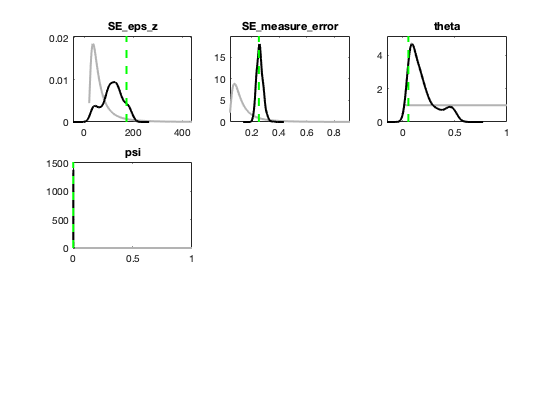
\includegraphics[scale=.8]{p5_priors_posteriors}

I think the estimated parameters are so different because this is a relatively simple model and does include a lot of important factors.

\end{document}



